\documentclass[10pt]{beamer}
\usepackage{pgf}
\usepackage{booktabs}
%Information to be included in the title page:
\title{Elite individuals, insitutions, and economic growth accounting}
\author{James Xu}
\institute{ECON 442, Duke University}
\date{2024}
\usefonttheme[onlymath]{serif}

\begin{document}
\setbeamertemplate{navigation symbols}{}

\frame{\titlepage}

\begin{frame}
    \frametitle{Research Question}
    \begin{block}{What is the relationship between elite students, academic institutions, and economic growth?}
        \begin{itemize}
            \item Are there outsized returns to economic growth when there are more academic elites?
            \item How can we measure academic competition and education quality beyond means?
        \end{itemize}
    \end{block}
    \begin{exampleblock}{Method}
        Through this paper, I investigate the relationship between the number of top-ranked universities, share of top math students,
        IMO scores, and GDP per capita growth to analyze these questions.
    \end{exampleblock}
\end{frame}

\begin{frame}
\frametitle{Data Sources}
\begin{itemize}
    \item World Bank: World Development Indicators
    \item International Math Olympiad
    \item ARWU University Rankings
    \item PISA Math Scores
    \item Economist Democracy Scores
\end{itemize}
\end{frame}

\begin{frame}{World Bank Data}
    The World Bank collects and publishes development indicators for most countries/economies in the world. In this paper, I use the following variables:

    \begin{itemize}
        \item GDP Per Capita Growth: \% growth in constant 2015 \$USD
        \item GDP Per Capita: current \$USD
        \item School Completion Rates: \% gross of relevant age group
        \begin{itemize}
            \item ``What \% of primary-school-aged population is enrolled in primary school?''
            \item This number can be greater than 100\%
            \item Not available for all years and all countries $\rightarrow$ missing data problem
        \end{itemize}
        \item Population: all residents of a country/territory
    \end{itemize}
\end{frame}

\begin{frame}
    \frametitle{World Bank Data}
    \framesubtitle{Distributions}
    \centering
    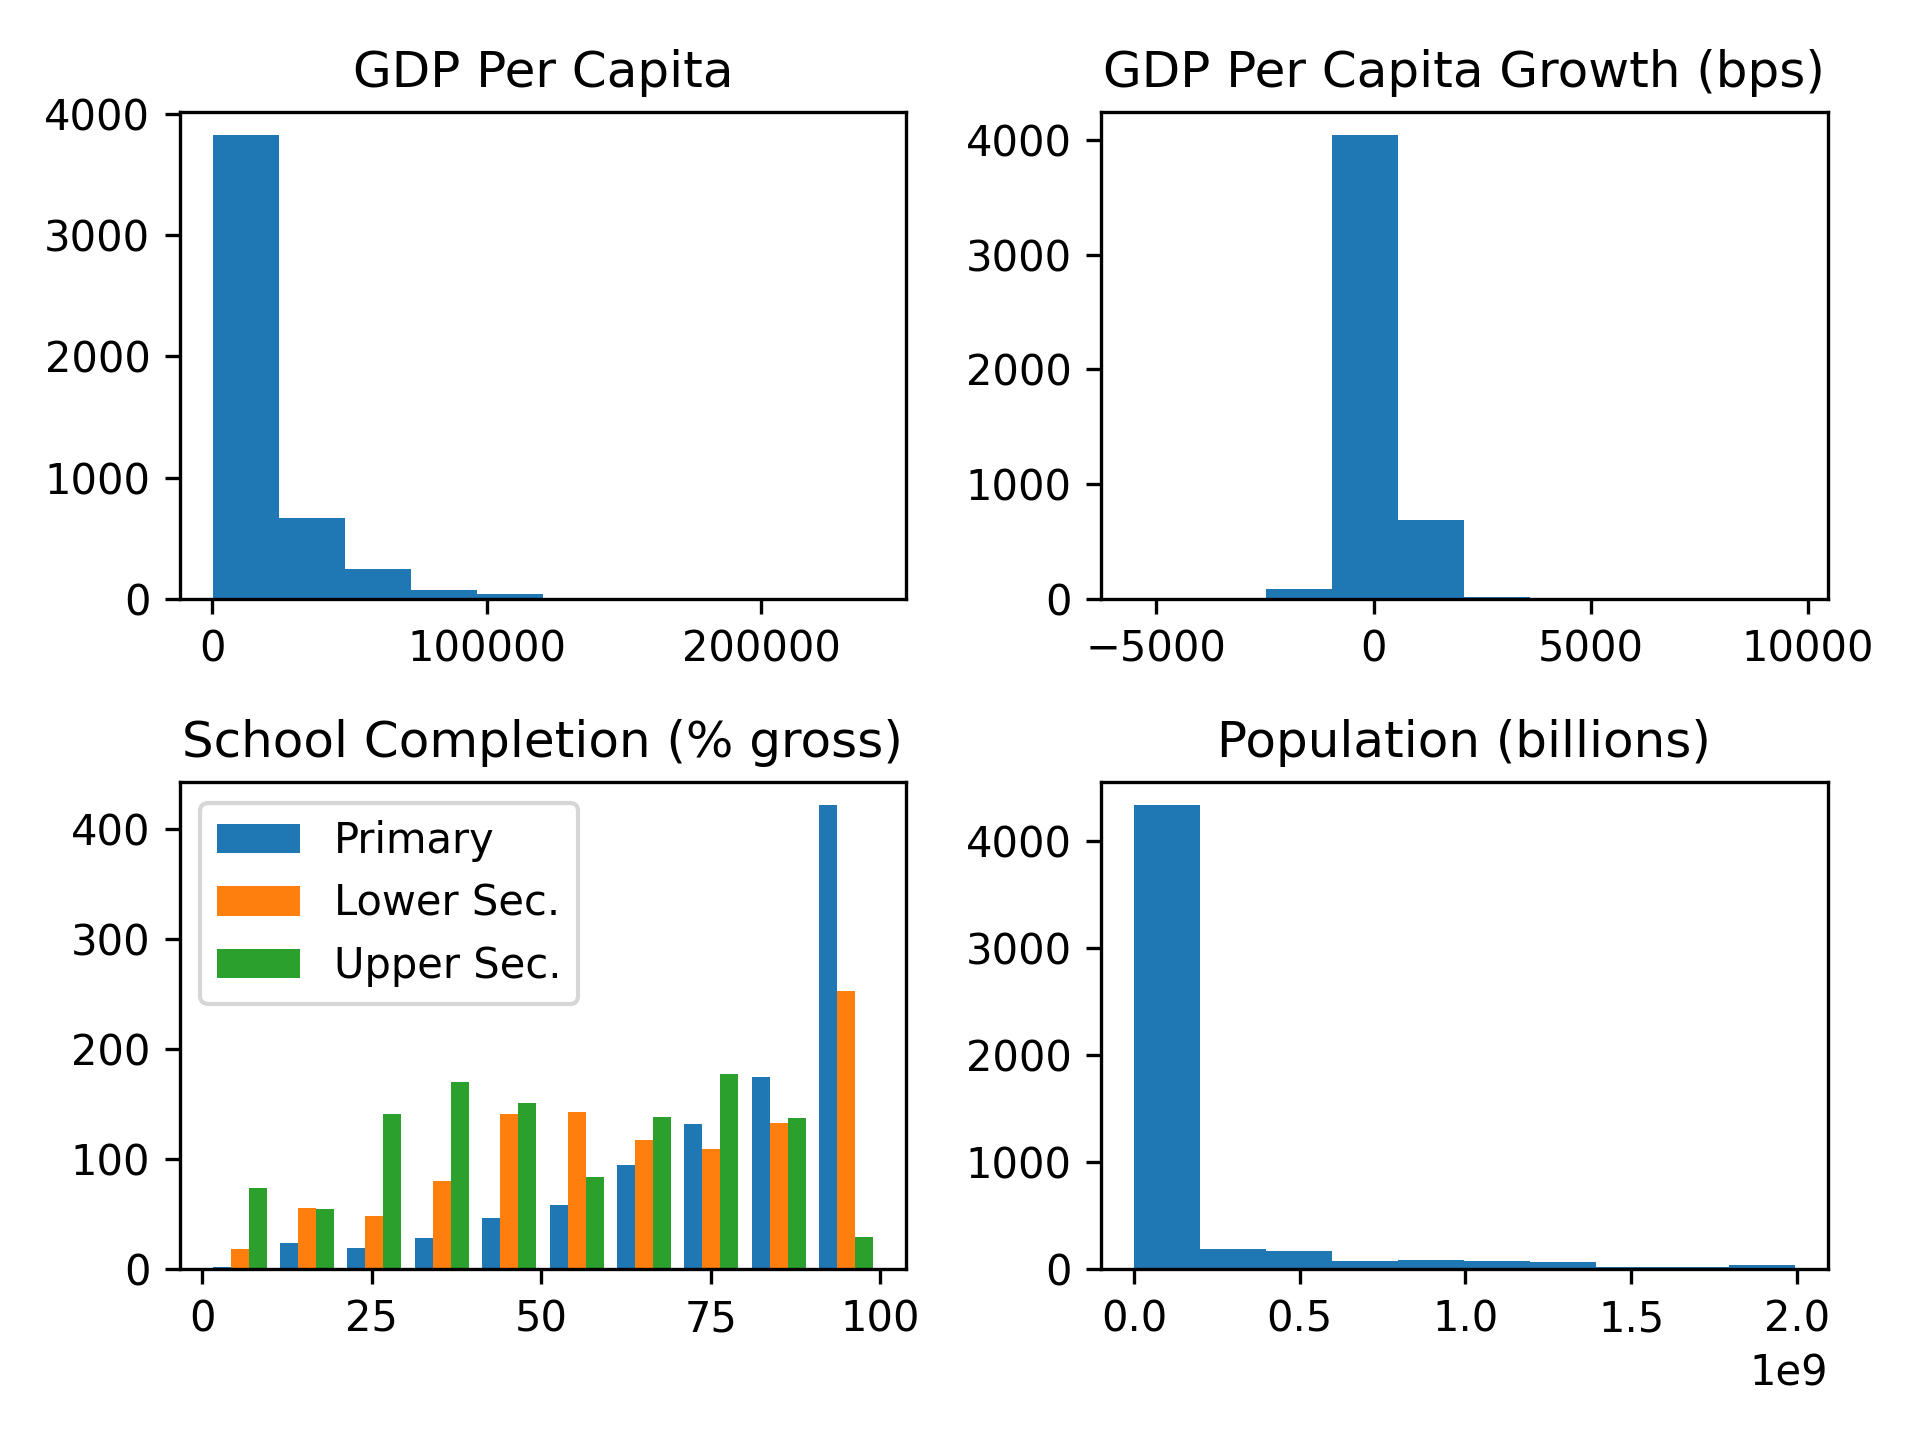
\includegraphics[width=\textwidth]{../charts/wdi.png}
\end{frame}

\begin{frame}
    \frametitle{World Bank Data}
    \framesubtitle{Missing data}
    \centering
    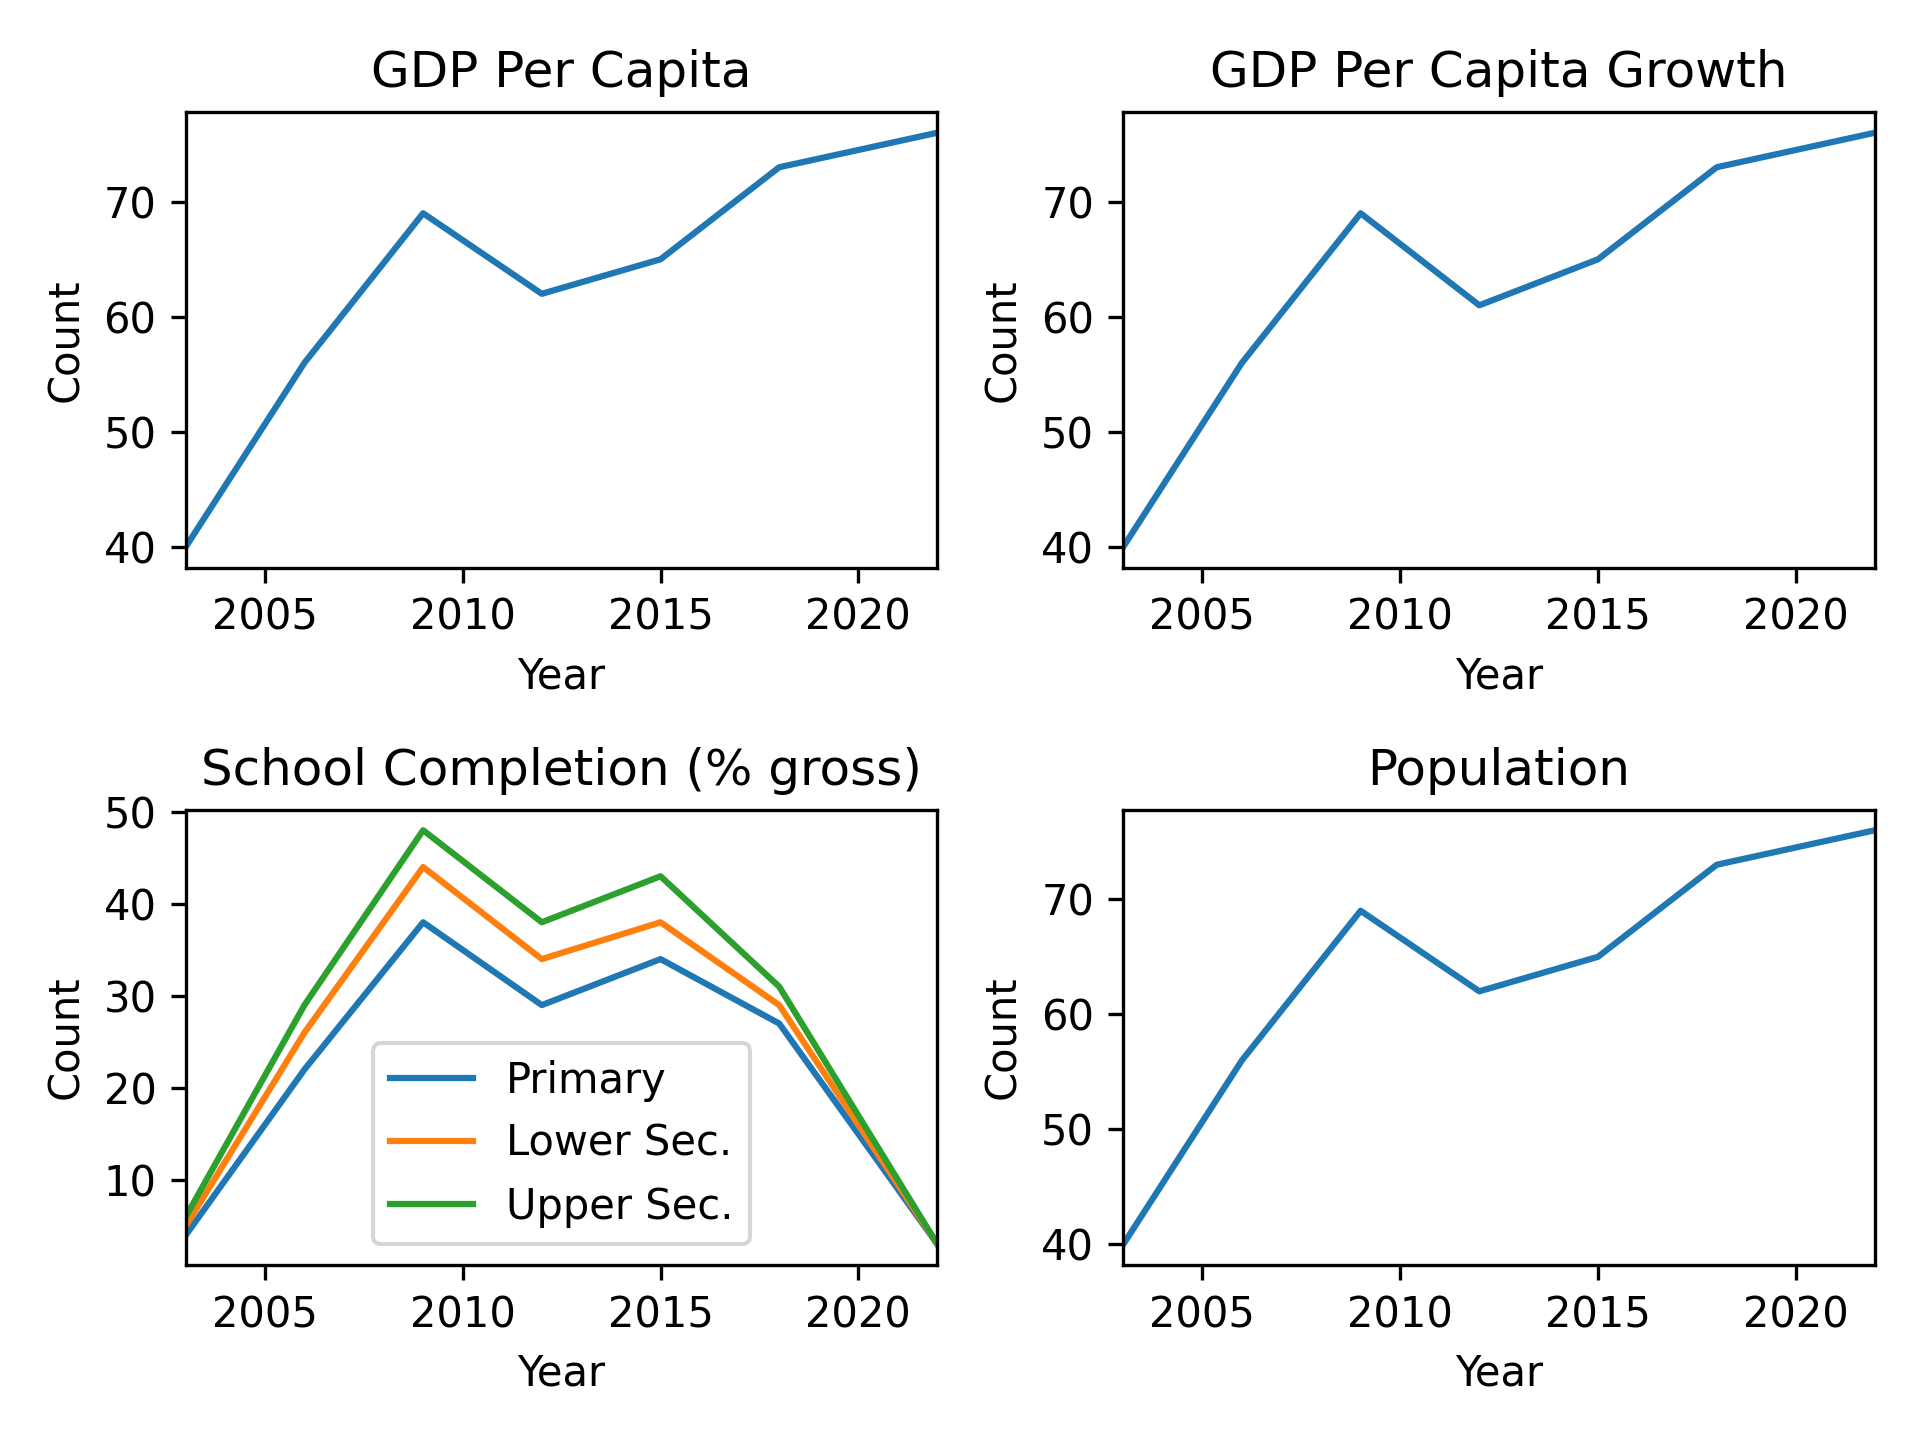
\includegraphics[width=\textwidth]{../charts/wdi-count.png}
\end{frame}

\begin{frame}{Imputing nulls}{Using XGBoost for better predictions}
    \begin{block}{Data is not missing at random}
        School completion data is only available for a maximum of 80 countries per year and has high variance in this availablility.
        This is the most limiting factor in the analysis.
    \end{block}

    \begin{block}{Predicting missing values}
        XGBoost is a tree-based model that has built-in null handling. I use the remaining variables to predict school completion rates and EIU democracy scores.
        Achieves significantly higher accuracy than linear regression.
    \end{block}
    
\end{frame}

\begin{frame}{Imputation results}{School completion rates}
    \centering
    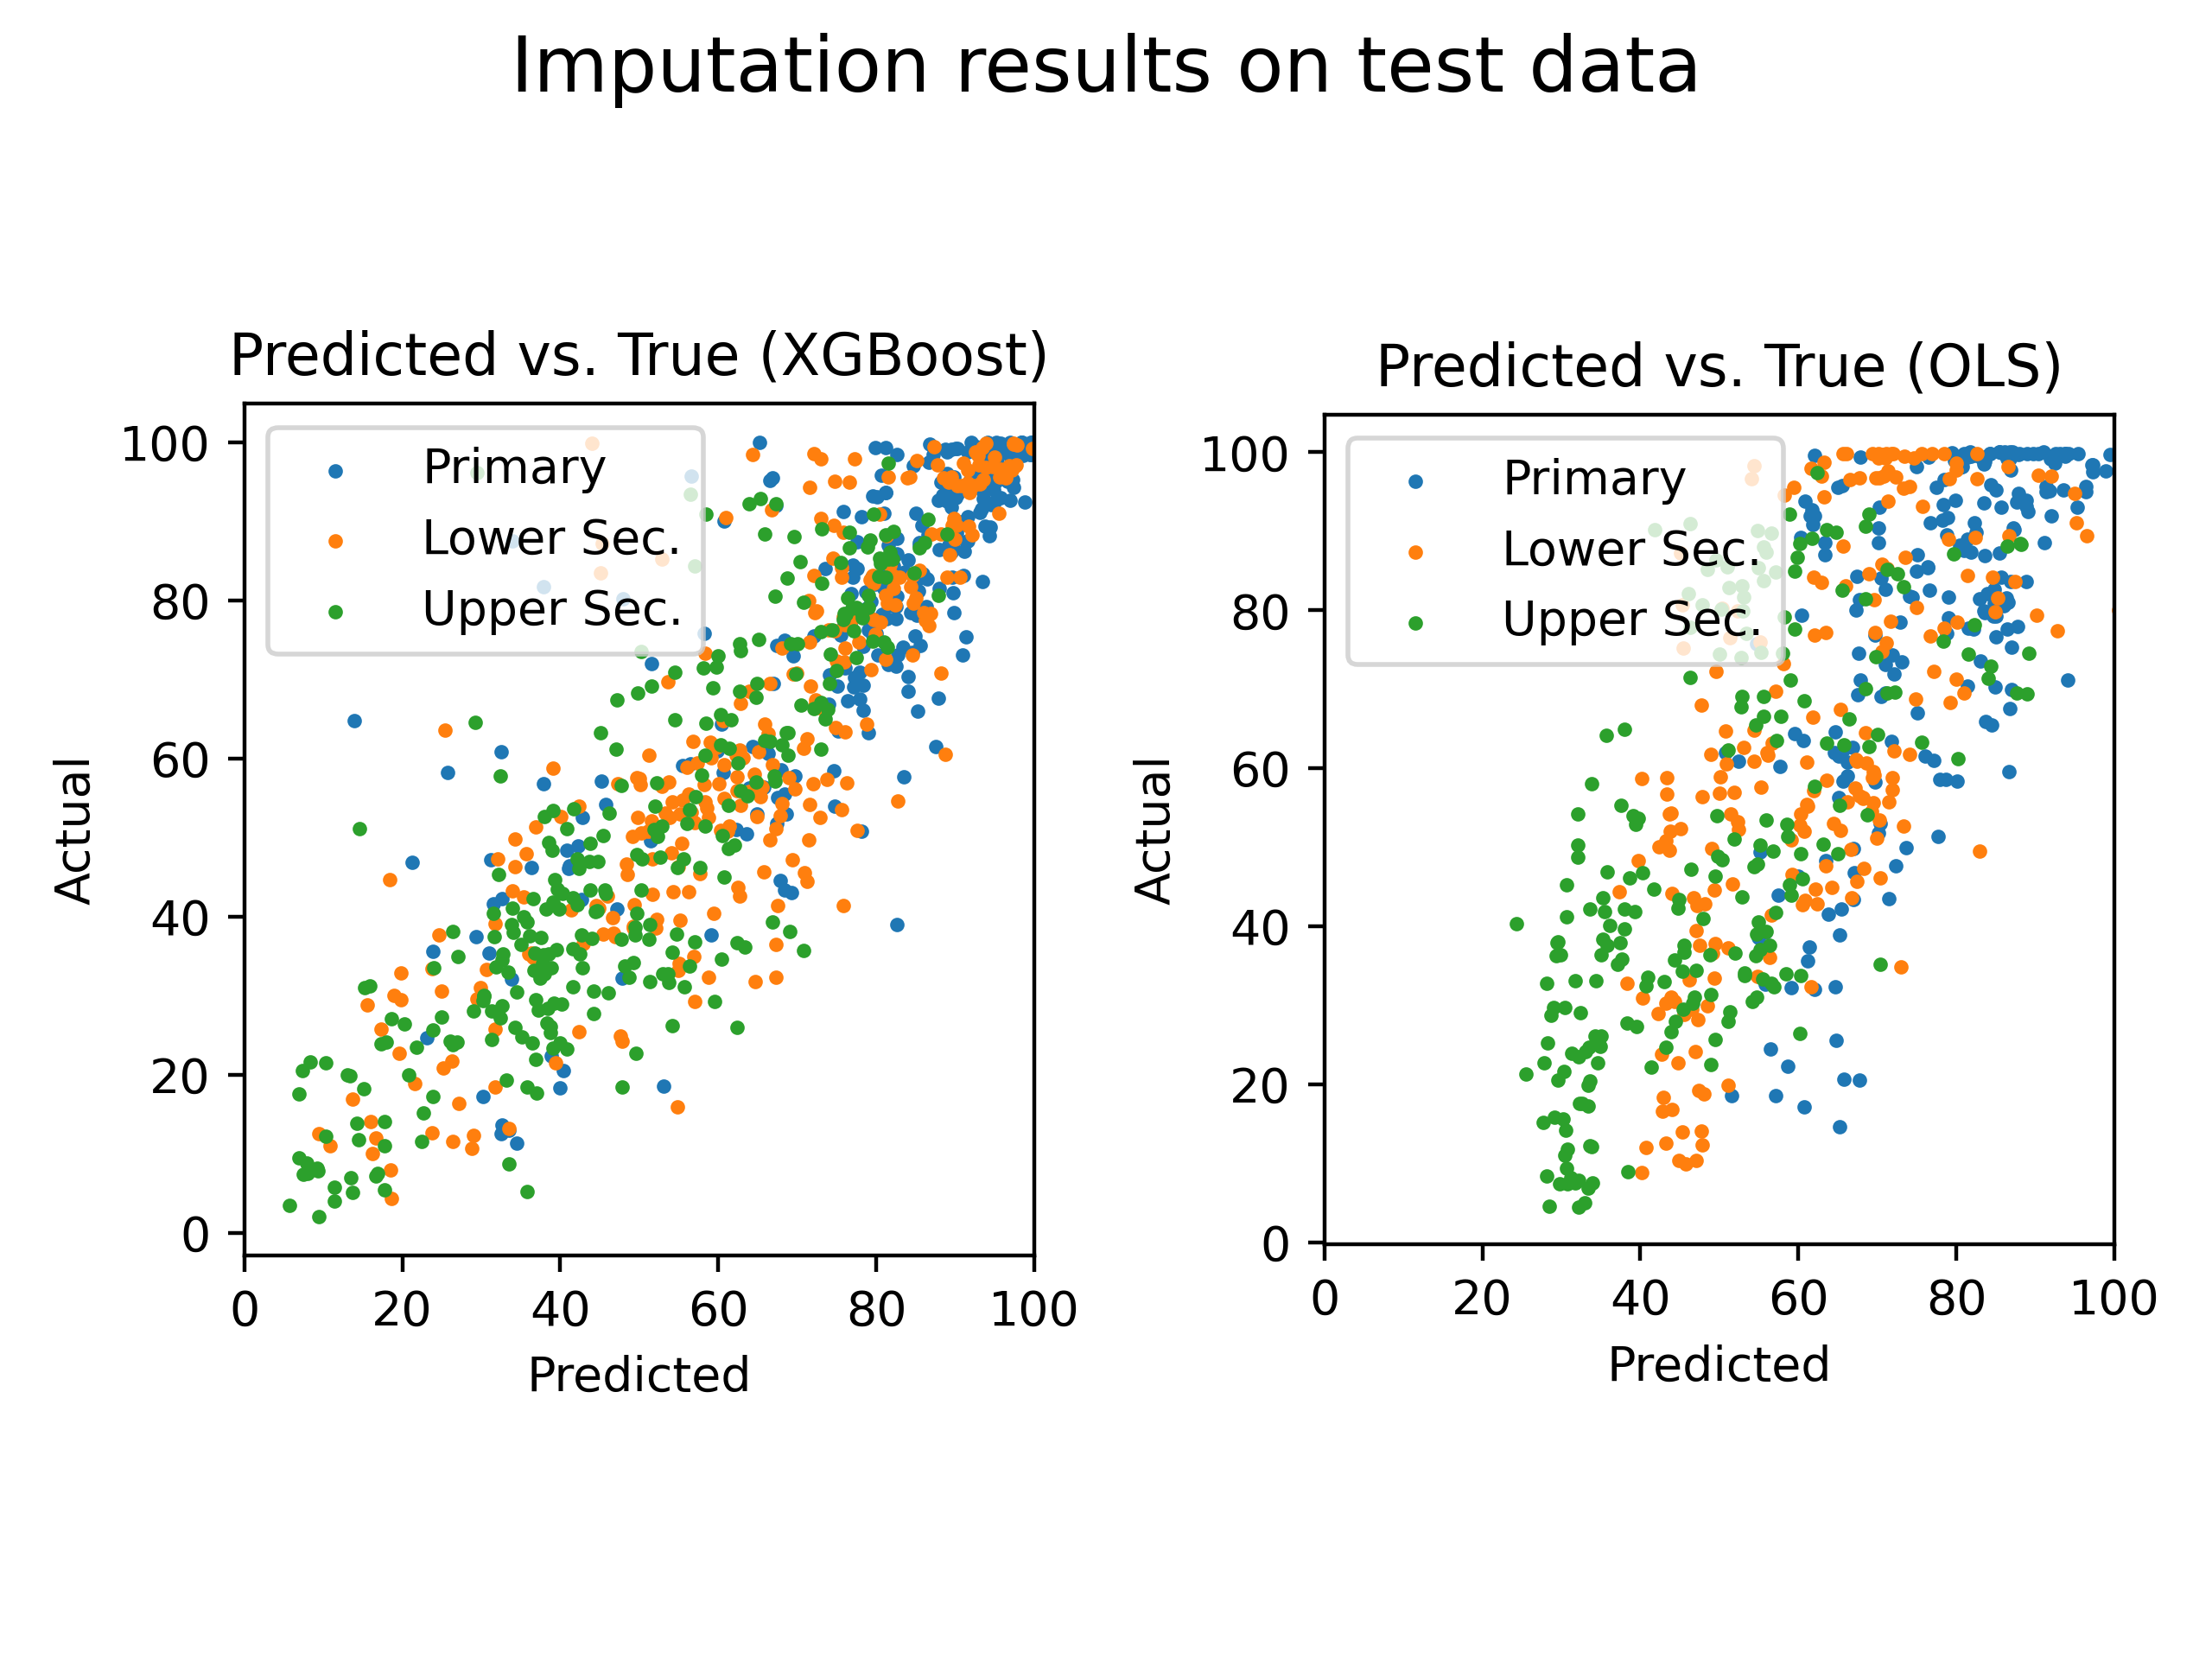
\includegraphics[width=\textwidth]{../build/xgboost.png}
\end{frame}

\begin{frame}{Imputation results}{EIU Democracy Score}
    \centering
    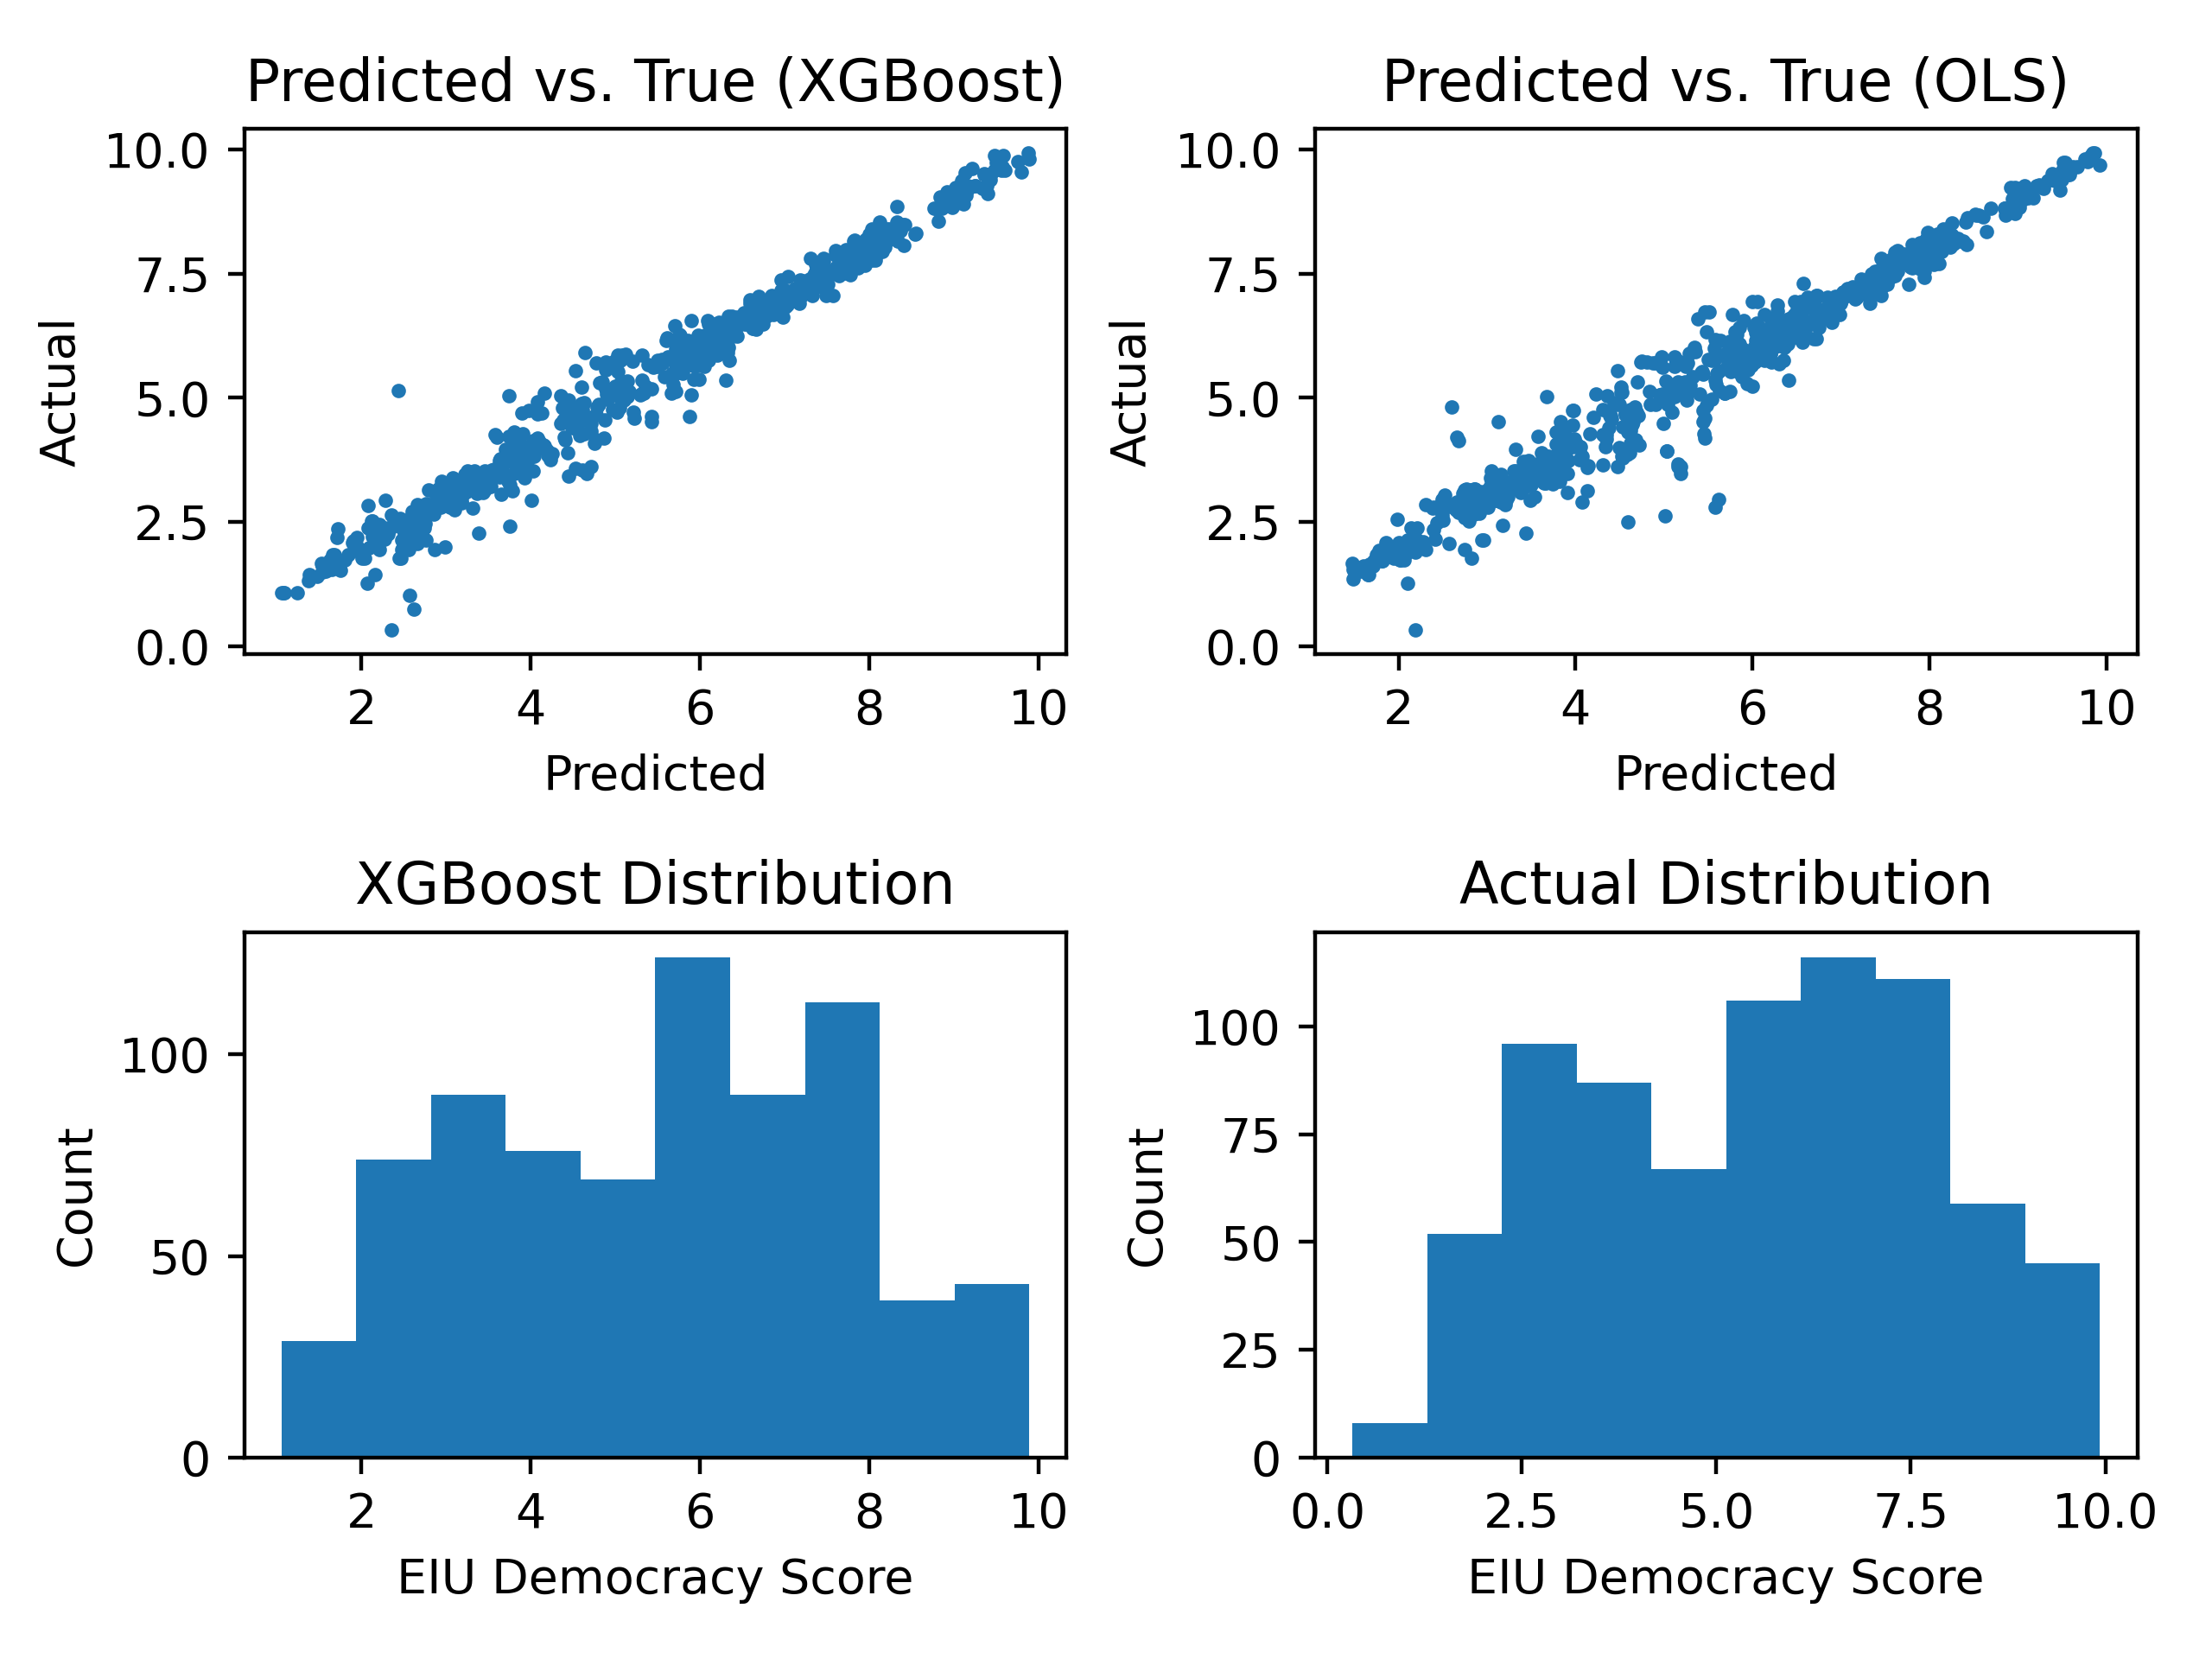
\includegraphics[width=\textwidth]{../build/eiu_xgboost.png}
\end{frame}

\begin{frame}{IMO Scores}{The IMO is an international mathematics contest for high school students
    }
    \begin{columns}
        \column{0.5\textwidth}
            \centering
            \begin{table}
            \caption{Top 10 countries by IMO score.}
            \resizebox{\textwidth}{!}{
            \begin{tabular}{lrrr}
                \toprule
                 & IMO Score & GDPpc & GDPpc Growth \\
                Region &  &  &  \\
                \midrule
                KOR & 10.2026 & 26060.9203 & 293.8552 \\
                CHN & 9.8296 & 6424.4972 & 786.8171 \\
                USA & 9.6196 & 54346.5078 & 125.7613 \\
                RUS & 9.0800 & 10432.8366 & 277.0704 \\
                SGP & 9.0642 & 51652.4651 & 348.0543 \\
                BGR & 8.8821 & 7556.3933 & 417.7564 \\
                ROU & 8.7367 & 9432.6698 & 439.7522 \\
                HUN & 8.7153 & 13979.7009 & 262.9650 \\
                VNM & 8.5029 & 2159.2583 & 527.6404 \\
                UKR & 8.3941 & 3079.8378 & 131.9303 \\
                \bottomrule
            \end{tabular}}
        \end{table}
        \column{0.5\textwidth}
            \begin{itemize}
                \item Scores collected from 2003 to 2022
                \item Scores are transformed by $t(s) = \frac{s}{\log P}$ where $s$ is the country's raw score and $P$ is population.
                \begin{itemize}
                    \item Team size of 6 means that larger countries have an advantage due to ``genius odds''
                    \item Score is capped, so dividing by $\log P$ will correct for theoretical ceiling of performance
                \end{itemize}
            \end{itemize}
        \end{columns}
\end{frame}

\begin{frame}{ARWU Rankings}{Description and Usage}
    ARWU (Academic Ranking of World Universities) is a set of university rankings based primarily on research output.
    \begin{itemize}
        \item Rankings are produced annually and are available from 2003
        \item From 2003 to 2016, 500 top universities were ranked; after 2017, 1000 were ranked.
    \end{itemize}
    
    \begin{block}{Per-Capita Scaling}
        Larger countries naturally have an advantage, so a more fair metric is
        \[ARWU_{i,t} = \frac{arwuCount_{i,t}}{P_{i,t}} \cdot 10^6 \]
        Instead, looking at ARWU insitutions per million population indicates the relative quantity of elite insitutions in a country/region.
    \end{block}
    
\end{frame}

\begin{frame}{Summary Statistics}
    Hello
\end{frame}

\begin{frame}{Rationale for variables}
    \begin{block}{IMO Scores}
        Indicator for a country's (and region's) ability to develop/identify pinncale STEM talent at high school level.
    \end{block}

    \begin{block}{ARWU Rankings}
        Indicator for a country's (and region's) ability to produce exellence in research output.
    \end{block}

    \begin{block}{Percent in PISA 99th percentile}
        When controlling for average PISA math scores, this is a partial indicator for whether general excellence in academics is encouraged/necessary.
    \end{block}
\end{frame}

\begin{frame}{Model specification}
    Let elite indicators be: $math99, ARWU, IMO$.
    For the sake of concision, let $E_{i,t}$ be a 1 by 4 matrix defined as:
    \[E_{i,t} = 
    \begin{bmatrix}
        math99_{i, t} & ARWU_{i, t} & ARWU_{i, t} \times GDPpc_{i, t} & IMO_{i, t}
    \end{bmatrix}
    \] for country/region $i$ in year $t$.
    Let the coefficients of $E_{i, t}$ be a 4 by 1 matrix called $\lambda$. For control variables, $I_{i, t}$ is the matrix of variables and $\alpha$ is coefficients.
    \begin{equation}
        Y_{i, t} = \beta_0 + \lambda E_{i, t} + \delta GDPpc \times E_{i,t} + \alpha I_{i, t} + T_t + C_i + \epsilon_{i, t}
    \end{equation}
    where $T,C$ represent time and entity dummies respectively and $Y_{i,t}$ be the GDP per capita growth in basis points for a country/region $i$ and year $t$.
\end{frame}

\begin{frame}{Relationships}
    \centering
    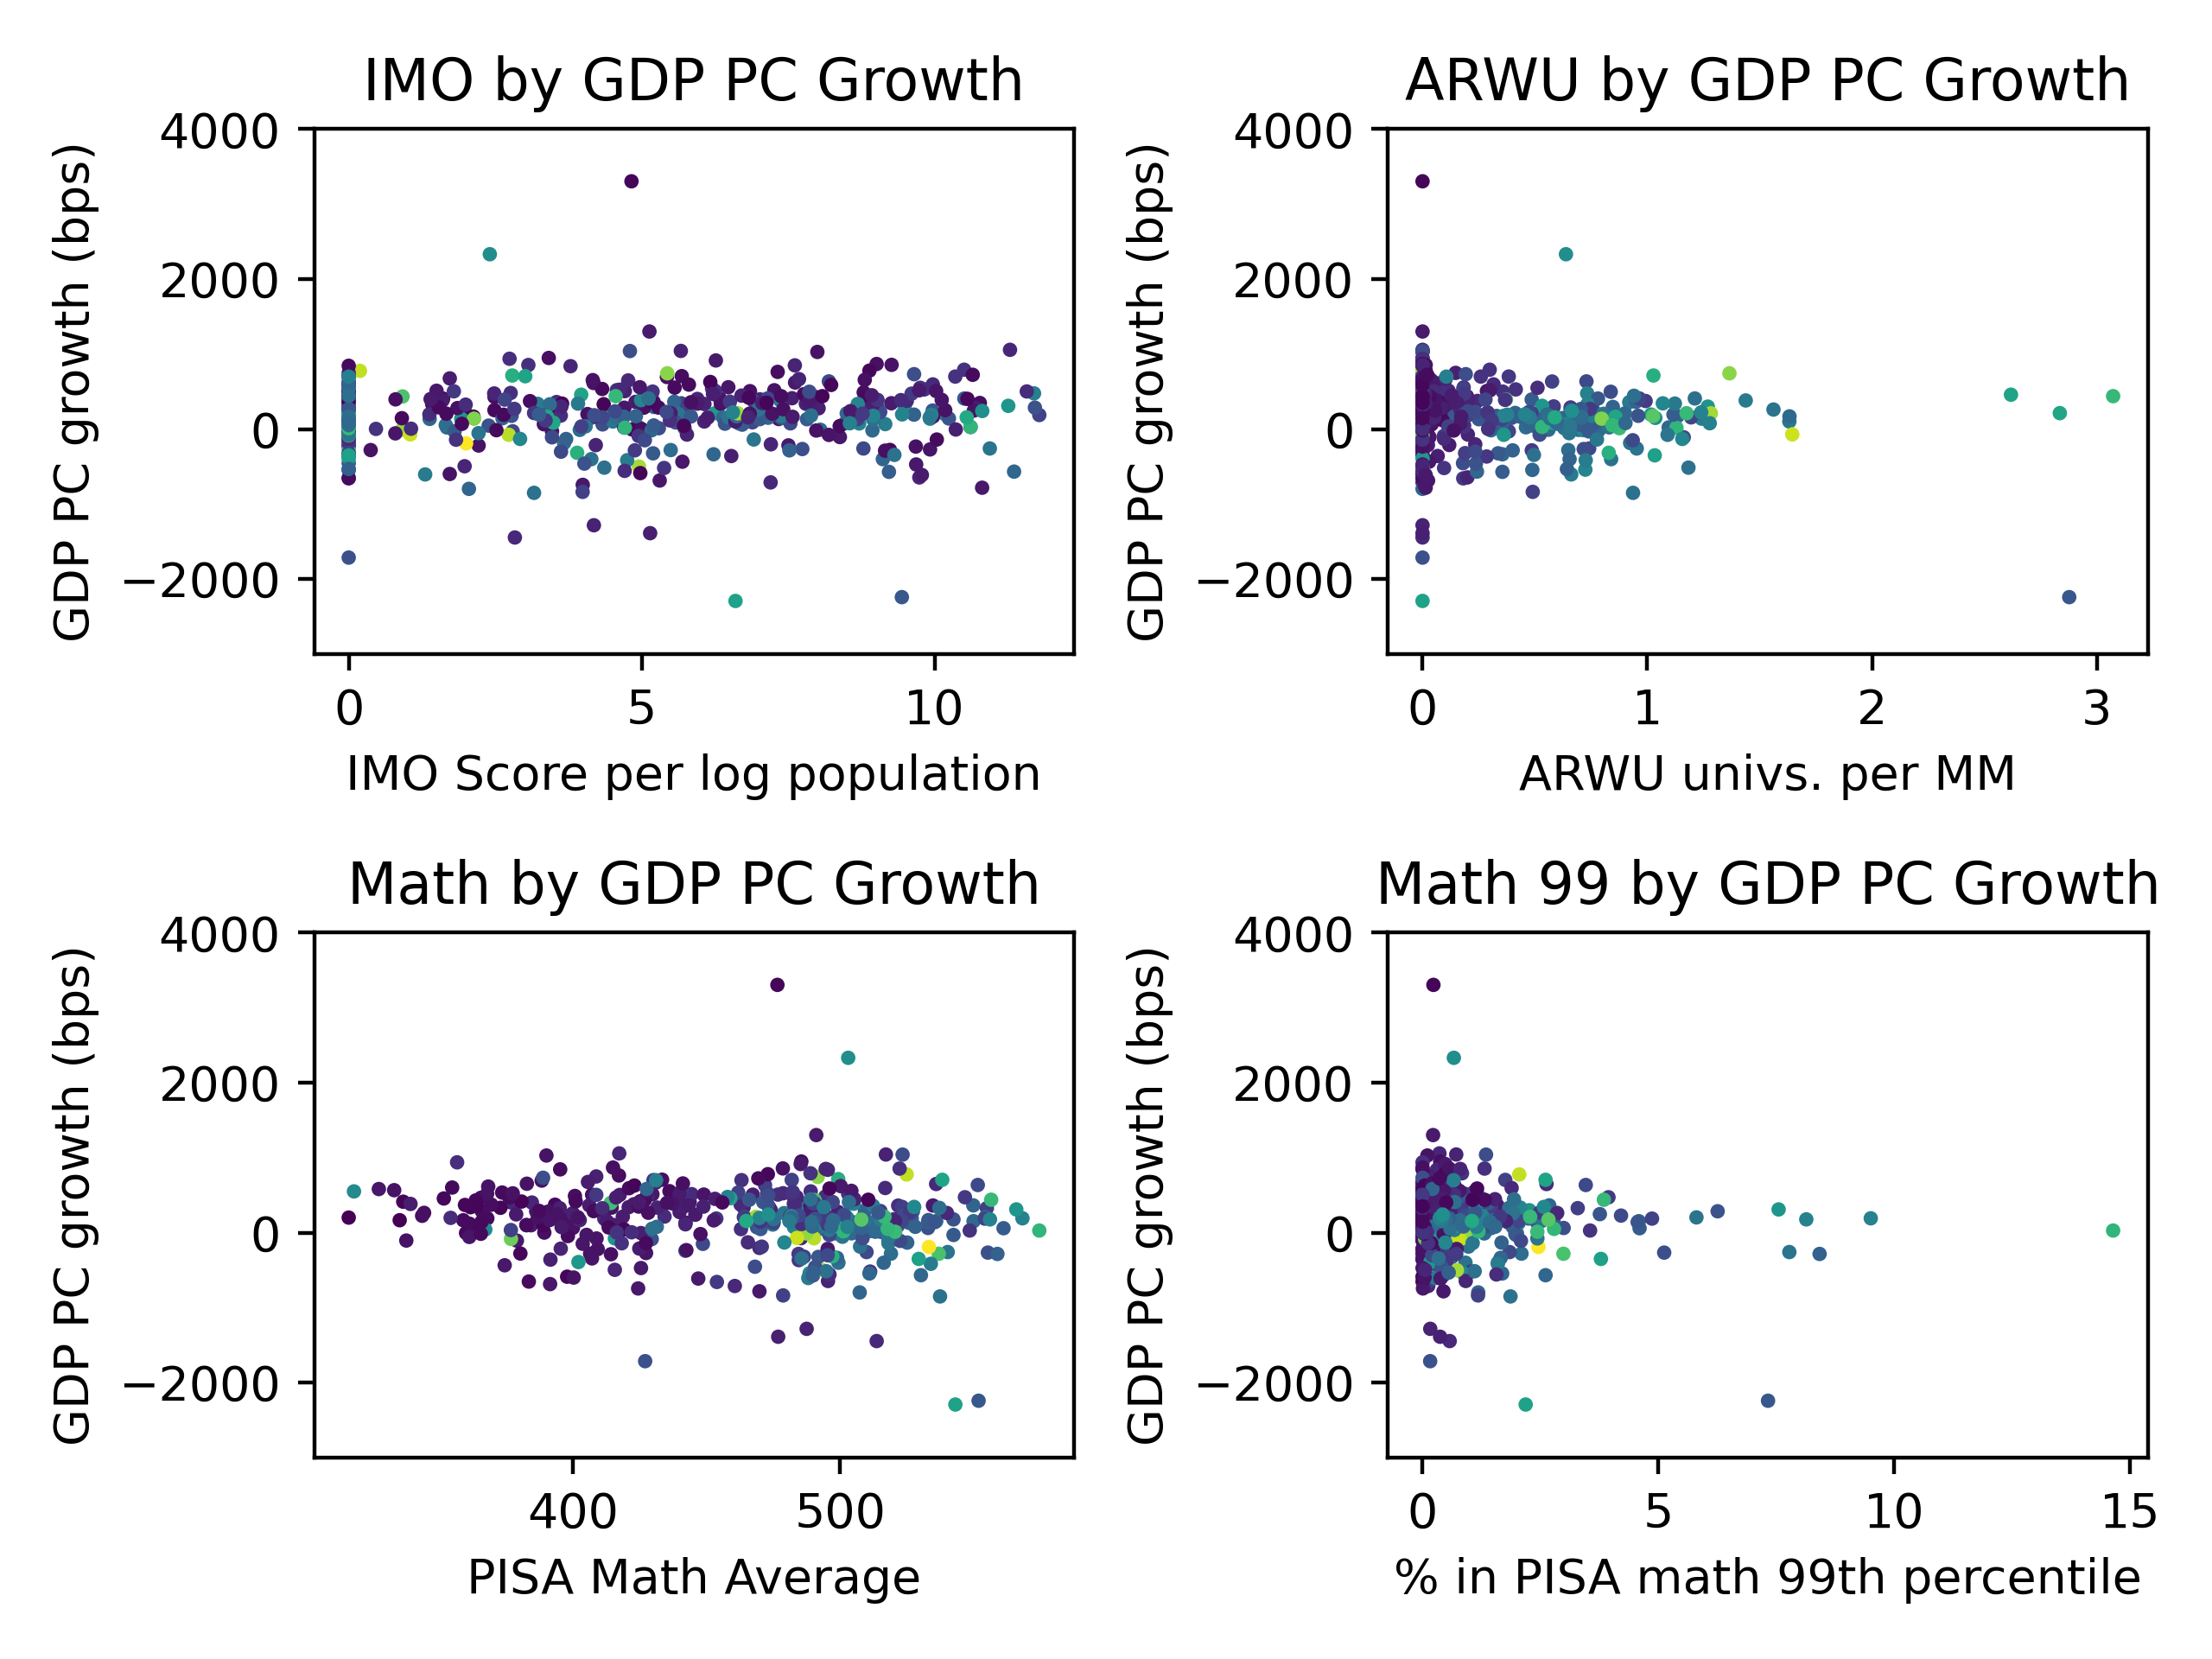
\includegraphics[width=\textwidth]{../charts/relationships.png}
\end{frame}

\begin{frame}{PISA panel regression}{Highly dependent on model specification due to rich country bias and limited variation}
    \begin{table}[!htbp] \centering
        \resizebox{\linewidth}{!} {
            \begin{tabular}{@{\extracolsep{5pt}}lcccc}
                \\[-1.8ex]\hline
                \hline \\[-1.8ex]
                & \multicolumn{4}{c}{\textit{Dependent variable: GDP Per Capita Growth (bps)}} \
                \cr \cline{2-5}
                \\[-1.8ex] & \multicolumn{1}{c}{Model 1 (base)} & \multicolumn{1}{c}{Model 2} & \multicolumn{1}{c}{Model 3 (Time FE)} & \multicolumn{1}{c}{Model 4 (Time + Entity FE)}  \\
                \hline \\[-1.8ex]
                 PISA Math in global P99 & & -43.491$^{}$ & -40.291$^{}$ & -126.152$^{*}$ \\
                & & (48.245) & (40.349) & (64.627) \\
                 PISA Math 99 x GDP PC & & 0.000$^{}$ & 0.000$^{}$ & 0.001$^{}$ \\
                & & (0.001) & (0.001) & (0.001) \\
                 IMO score per log population & 6.604$^{}$ & 3.629$^{}$ & 4.581$^{}$ & 20.285$^{}$ \\
                & (8.473) & (10.582) & (8.833) & (21.169) \\
                 IMO score x GDP pc & -0.000$^{}$ & 0.000$^{}$ & -0.000$^{}$ & -0.001$^{*}$ \\
                & (0.000) & (0.000) & (0.000) & (0.000) \\
                 ARWU insitutions & -588.767$^{***}$ & -538.997$^{***}$ & -580.030$^{***}$ & -764.617$^{***}$ \\
                & (135.656) & (178.746) & (149.452) & (250.804) \\
                 ARWU insitutions x GDP PC & 0.009$^{***}$ & 0.008$^{**}$ & 0.009$^{***}$ & 0.011$^{***}$ \\
                & (0.003) & (0.003) & (0.003) & (0.004) \\
                 PISA Math & & 1.150$^{}$ & 0.908$^{}$ & 0.495$^{}$ \\
                & & (0.792) & (0.732) & (1.761) \\
                 GDP per capita & -0.003$^{**}$ & -0.003$^{*}$ & -0.003$^{**}$ & 0.000$^{}$ \\
                & (0.001) & (0.002) & (0.001) & (0.005) \\
                 Primary School Completion Rate & -3.554$^{}$ & -11.911$^{***}$ & -5.387$^{}$ & -4.028$^{}$ \\
                & (3.345) & (4.157) & (3.602) & (4.947) \\
                 Lower Sec. Completion Rate & -1.475$^{}$ & -0.571$^{}$ & -1.291$^{}$ & -0.446$^{}$ \\
                & (2.945) & (3.540) & (2.948) & (4.443) \\
                 Upper Sec. Completion Rate & 5.643$^{**}$ & 6.665$^{**}$ & 5.385$^{**}$ & 3.364$^{}$ \\
                & (2.343) & (2.835) & (2.354) & (3.692) \\
                 Democracy Rating & -1.606$^{}$ & 2.270$^{}$ & -7.429$^{}$ & 36.204$^{}$ \\
                & (13.894) & (17.254) & (14.431) & (61.854) \\
                 Time Effects & Yes & No & Yes & Yes \\
                 Fixed Effects & No & No & No & Yes \\
                 Entities & 89 & 89 & 89 & 89 \\
                \hline \\[-1.8ex]
                 Observations & 440 & 440 & 440 & 440 \\
                 $R^2$ & 0.388 & 0.092 & 0.392 & 0.567 \\
                 Adjusted $R^2$ & 0.364 & 0.064 & 0.364 & 0.428 \\
                 Residual Std. Error & 360.908 (df=423) & 437.923 (df=426) & 360.976 (df=420) & 342.461 (df=332) \\
                 F Statistic & 16.727$^{***}$ (df=16; 423) & 3.314$^{***}$ (df=13; 426) & 14.230$^{***}$ (df=19; 420) & 4.066$^{***}$ (df=107; 332) \\
                \hline
                \hline \\[-1.8ex]
                \textit{Note:} & \multicolumn{4}{r}{$^{*}$p$<$0.1; $^{**}$p$<$0.05; $^{***}$p$<$0.01} \\
                \end{tabular}
        }
        \end{table}
\end{frame}

\begin{frame}{PISA yearly regression}
    \begin{table}[!htbp] \centering
        \resizebox{\linewidth}{!} {
            \begin{tabular}{@{\extracolsep{1pt}}lcccccccc}
                \\[-1.8ex]\hline
                \hline \\[-1.8ex]
                & \multicolumn{8}{c}{\textit{Dependent variable: GDP Per Capita Growth (bps)}} \
                \cr \cline{2-9}
                \\[-1.8ex] & \multicolumn{1}{c}{2003} & \multicolumn{1}{c}{2006} & \multicolumn{1}{c}{2009} & \multicolumn{1}{c}{2012} & \multicolumn{1}{c}{2015} & \multicolumn{1}{c}{2018} & \multicolumn{1}{c}{2022} & \multicolumn{1}{c}{Panel FE}  \\
                \hline \\[-1.8ex]
                 PISA Math in global P99 & -36.263$^{}$ & -323.594$^{**}$ & 128.012$^{}$ & -57.807$^{}$ & 466.275$^{**}$ & -13.249$^{}$ & -185.929$^{**}$ & -126.152$^{*}$ \\
                & (92.257) & (138.527) & (134.080) & (93.739) & (198.856) & (80.330) & (75.932) & (64.627) \\
                 PISA Math 99 x GDP PC & -0.000$^{}$ & 0.004$^{}$ & 0.001$^{}$ & 0.001$^{}$ & -0.009$^{**}$ & 0.000$^{}$ & 0.002$^{}$ & 0.001$^{}$ \\
                & (0.002) & (0.003) & (0.003) & (0.002) & (0.004) & (0.001) & (0.001) & (0.001) \\
                 IMO score per log population & 5.787$^{}$ & 13.706$^{}$ & 7.250$^{}$ & 9.955$^{}$ & 27.849$^{}$ & 2.586$^{}$ & -10.574$^{}$ & 20.285$^{}$ \\
                & (24.329) & (28.793) & (25.375) & (20.089) & (37.305) & (10.918) & (18.736) & (21.169) \\
                 IMO score x GDP pc & -0.000$^{}$ & -0.001$^{}$ & 0.000$^{}$ & 0.000$^{}$ & -0.001$^{}$ & -0.000$^{}$ & 0.000$^{}$ & -0.001$^{*}$ \\
                & (0.001) & (0.001) & (0.001) & (0.001) & (0.001) & (0.000) & (0.000) & (0.000) \\
                 ARWU insitutions & -461.941$^{}$ & -374.847$^{}$ & 298.772$^{}$ & -746.052$^{**}$ & -1132.300$^{}$ & -365.119$^{}$ & -1310.810$^{***}$ & -764.617$^{***}$ \\
                & (443.713) & (420.235) & (453.763) & (292.719) & (718.477) & (288.492) & (455.353) & (250.804) \\
                 ARWU insitutions x GDP PC & 0.004$^{}$ & 0.001$^{}$ & -0.004$^{}$ & 0.008$^{}$ & 0.030$^{**}$ & 0.006$^{}$ & 0.013$^{}$ & 0.011$^{***}$ \\
                & (0.011) & (0.009) & (0.009) & (0.005) & (0.014) & (0.004) & (0.008) & (0.004) \\
                 PISA Math & 0.436$^{}$ & 6.935$^{***}$ & -6.860$^{***}$ & 0.324$^{}$ & -1.519$^{}$ & 1.177$^{}$ & 2.807$^{}$ & 0.495$^{}$ \\
                & (1.552) & (1.906) & (2.386) & (1.489) & (2.828) & (1.002) & (2.056) & (1.761) \\
                 GDP per capita & -0.006$^{}$ & -0.005$^{}$ & -0.000$^{}$ & -0.003$^{}$ & 0.002$^{}$ & -0.007$^{***}$ & -0.003$^{}$ & 0.000$^{}$ \\
                & (0.005) & (0.005) & (0.006) & (0.002) & (0.005) & (0.002) & (0.004) & (0.005) \\
                 Primary School Completion Rate & 7.306$^{}$ & -11.680$^{}$ & 4.589$^{}$ & -15.665$^{}$ & -4.820$^{}$ & -8.787$^{}$ & 4.752$^{}$ & -4.028$^{}$ \\
                & (4.789) & (10.409) & (13.405) & (9.658) & (14.437) & (5.579) & (9.745) & (4.947) \\
                 Lower Sec. Completion Rate & 4.652$^{}$ & 7.506$^{}$ & -0.454$^{}$ & 2.430$^{}$ & -1.228$^{}$ & 6.617$^{*}$ & -13.439$^{}$ & -0.446$^{}$ \\
                & (6.867) & (8.157) & (8.302) & (5.785) & (10.676) & (3.951) & (8.396) & (4.443) \\
                 Upper Sec. Completion Rate & 4.916$^{}$ & 3.930$^{}$ & -2.992$^{}$ & 5.781$^{}$ & 4.631$^{}$ & 0.908$^{}$ & 10.924$^{*}$ & 3.364$^{}$ \\
                & (7.172) & (6.850) & (7.450) & (4.375) & (8.029) & (3.174) & (6.081) & (3.692) \\
                 Democracy Rating & -91.681$^{**}$ & -148.435$^{**}$ & 59.739$^{}$ & 36.375$^{}$ & 25.423$^{}$ & 15.183$^{}$ & -5.316$^{}$ & 36.204$^{}$ \\
                & (39.476) & (56.849) & (46.067) & (30.648) & (51.072) & (16.370) & (28.766) & (61.854) \\
                \hline \\[-1.8ex]
                 Observations & 40 & 56 & 69 & 61 & 65 & 73 & 76 & 440 \\
                 $R^2$ & 0.677 & 0.536 & 0.268 & 0.363 & 0.267 & 0.343 & 0.477 & 0.567 \\
                 Adjusted $R^2$ & 0.516 & 0.392 & 0.095 & 0.187 & 0.081 & 0.198 & 0.368 & 0.428 \\
                 Residual Std. Error & 188.826 (df=26) & 363.704 (df=42) & 411.759 (df=55) & 250.551 (df=47) & 455.710 (df=51) & 178.763 (df=59) & 325.047 (df=62) & 342.461 (df=332) \\
                 F Statistic & 4.193$^{***}$ (df=13; 26) & 3.732$^{***}$ (df=13; 42) & 1.547$^{}$ (df=13; 55) & 2.060$^{**}$ (df=13; 47) & 1.432$^{}$ (df=13; 51) & 2.365$^{**}$ (df=13; 59) & 4.353$^{***}$ (df=13; 62) & 4.066$^{***}$ (df=107; 332) \\
                \hline
                \hline \\[-1.8ex]
                \textit{Note:} & \multicolumn{8}{r}{$^{*}$p$<$0.1; $^{**}$p$<$0.05; $^{***}$p$<$0.01} \\
                \end{tabular}
        }
        \end{table}
        
\end{frame}

% \begin{frame}
%     \frametitle{Non-PISA data regression}
%     \begin{table}[!htbp] \centering
%         \resizebox{\linewidth}{!} {
%             \begin{tabular}{@{\extracolsep{5pt}}lcccc}
%                 \\[-1.8ex]\hline
%                 \hline \\[-1.8ex]
%                 & \multicolumn{4}{c}{\textit{Dependent variable: GDPpcGrowth}} \
%                 \cr \cline{2-5}
%                 \\[-1.8ex] & \multicolumn{1}{c}{Model 3 (PISA)} & \multicolumn{1}{c}{Model 5 (PISA years)} & \multicolumn{1}{c}{Model 6 (All years)} & \multicolumn{1}{c}{Model 7 (All years, FE)}  \\
%                 \hline \\[-1.8ex]
%                  IMO score per log population & 10.055$^{}$ & 18.160$^{***}$ & 13.297$^{***}$ & 10.006$^{}$ \\
%                 & (8.154) & (6.517) & (3.993) & (10.776) \\
%                  ARWU insitutions & -575.550$^{***}$ & -446.996$^{**}$ & -353.730$^{***}$ & 523.241$^{*}$ \\
%                 & (213.365) & (221.189) & (131.179) & (292.381) \\
%                  ARWU insitutions x GDP PC & 0.008$^{*}$ & 0.008$^{*}$ & 0.005$^{*}$ & -0.012$^{**}$ \\
%                 & (0.004) & (0.004) & (0.002) & (0.006) \\
%                  GDP per capita & -0.004$^{**}$ & -0.005$^{***}$ & -0.004$^{***}$ & 0.002$^{}$ \\
%                 & (0.002) & (0.002) & (0.001) & (0.004) \\
%                  Primary School Completion Rate & -0.112$^{}$ & -3.530$^{**}$ & -1.754$^{}$ & -1.505$^{}$ \\
%                 & (4.338) & (1.740) & (1.227) & (4.983) \\
%                  Lower Sec. Completion Rate & 1.568$^{}$ & 5.370$^{**}$ & 1.911$^{}$ & -0.147$^{}$ \\
%                 & (3.290) & (2.445) & (1.692) & (5.035) \\
%                  Upper Sec. Completion Rate & 1.542$^{}$ & -2.365$^{}$ & 0.081$^{}$ & 1.981$^{}$ \\
%                 & (2.543) & (1.946) & (1.325) & (3.776) \\
%                  Democracy Rating & 4.167$^{}$ & 13.397$^{}$ & 19.784$^{***}$ & 87.626$^{**}$ \\
%                 & (21.249) & (11.913) & (7.637) & (37.349) \\
%                  Population & -0.000$^{*}$ & -0.000$^{}$ & -0.000$^{}$ & 0.000$^{}$ \\
%                 & (0.000) & (0.000) & (0.000) & (0.000) \\
%                  Time Effects & Yes & Yes & Yes & Yes \\
%                  Fixed Effects & No & No & No & Yes \\
%                  Entities & 48 & 103 & 137 & 137 \\
%                 \hline \\[-1.8ex]
%                  Observations & 109 & 222 & 746 & 746 \\
%                  $R^2$ & 0.402 & 0.202 & 0.380 & 0.611 \\
%                  Adjusted $R^2$ & 0.313 & 0.156 & 0.360 & 0.505 \\
%                  Residual Std. Error & 199.076 (df=94) & 240.456 (df=209) & 288.864 (df=722) & 253.976 (df=586) \\
%                  F Statistic & 4.512$^{***}$ (df=14; 94) & 4.417$^{***}$ (df=12; 209) & 19.219$^{***}$ (df=23; 722) & 5.785$^{***}$ (df=159; 586) \\
%                 \hline
%                 \hline \\[-1.8ex]
%                 \textit{Note:} & \multicolumn{4}{r}{$^{*}$p$<$0.1; $^{**}$p$<$0.05; $^{***}$p$<$0.01} \\
%             \end{tabular}
%         }
%         \end{table}
% \end{frame}

\begin{frame}{Interpretation}
    \begin{block}{IMO Scores}
        \begin{itemize}
            \item Mostly indicates positive main relationship with GDP per capita growth, but negative interaction with GDP per capita.
            \item Suggests that lower income countries may see more benefit to what IMO scores are a proxy of (non-causal)
        \end{itemize}
    \end{block}

    \begin{block}{PISA math 99 percentile share}
        \begin{itemize}
            \item Very sensitive to model specification and changes between years
            \item Negative main effect but positive interaction effect
        \end{itemize}
    \end{block}

    \begin{block}{ARWU insitutions per million}
        \begin{itemize}
            \item Consistent negative main effect, but positive interaction effect with GDP per capita
            \item Can interpret as OVB, or that higher income countries may see more use from high-ranking institutions
        \end{itemize}
    \end{block}
    
\end{frame}

\begin{frame}{Limitations: data sample problems}
    Regression results do not present a clear picture of the existence of a statistical relationship between elite indicators and economic growth.
    \begin{block}{Little variation in data}
        \begin{itemize}
            \item Countries and regions with PISA test scores tend to be wealthier, more developed economies
            \item Low variance within countries over time and between countries as a result
        \end{itemize}
    \end{block}

    \begin{block}{Model specification matters}
        \begin{itemize}
            \item Including entity fixed effects makes the most significant difference versus time effects (likely due to above)
            \item Magnitudes of $math99$ is 10x larger when entity fixed effects are included; similar for $IMO$
            \item $ARWU$ and interaction terms reversed in sign compared to not including fixed effects
            \begin{itemize}
                \item Possibly due to omitted variable bias that is captured by fixed effects
            \end{itemize}
        \end{itemize}

    \end{block}
    
\end{frame}

\begin{frame}{Limitations: Yearly vs. Panel}{Significant year-to-year variation}
    \begin{block}{Unstable panel vs. yearly results}
        The panel methods mask some of the year-to-year changes in relationships.
        Some indicators are more stable than others, but $math99$ in particular alternates from positive to negative coefficient with large swings.
    \end{block}

    \begin{block}{Omitted Variable Bias}
        Large changes in relationship magnitude and direction suggests that omitted variable bias is a big problem.
    \end{block}
    
    
\end{frame}

\end{document}